\providecommand\ExamFontPath{../../../字体/}
\documentclass[fontset=exam]{exam-zh}
\usepackage{longtable,booktabs,array,calc,multirow,fvextra}
\usepackage[normalem]{ulem}
\providecommand{\hl}[1]{#1}
\providecommand{\ul}[1]{\uline{#1}}
\DefineVerbatimEnvironment{verbatim}{Verbatim}{breaklines=true,fontsize=\small}
\providecommand{\tightlist}{\setlength{\itemsep}{0pt}\setlength{\parskip}{0pt}}
\newcommand{\pandocbounded}[1]{#1}
\setlength{\emergencystretch}{3em}
\setlength{\tabcolsep}{2pt}
\examsetup{page/size=a4paper}
\title{厦门大学 2012—2013 年 期中考试}
\subject[4em]{热学}
\begin{document}
\maketitle
\fancyfoot[C]{第 \thepage 页（共 \pageref*{LastPage} 页）}
1．（14 分）

（1）从宏观上看，什么是温度？从微观上看，温度的统计意义是什么？

（2）根据分子动理论，气体的压强如何产生？写出理想气体的压强与分子数密度和分子平均平动动能的关系。

2．（16 分）

一打气筒，每打一次气可将原来压强为\(p_{0} = 1.0\text{a}\text{t}\text{m}\)，温度为\(t_{0} = 27.0^{0}\text{C}\)，体积\(V_{0} = 4.0\text{L}\)的空气压缩到容器内。设容器的体积\(V = 1.5 \times 10^{3}\text{L}\)，打气之前容器内空气的压强和温度分别为\(p_{0}\)和\(t_{0}\)。问要大打几次气才能使容器内空气的温度为\(t = 45^{0}\text{C}\)，压强为\(p = 2.0\text{a}\text{t}\text{m}\)？

3.（18 分）

容器中储存有 2mol 压强为\emph{p}＝6.9×10\textsuperscript{5}Pa，温度\emph{t}＝127\textsuperscript{0}C 的氧气，求：

（1）单位体积的分子数；

（2）一个分子的平均平动动能；

（3）系统的内能；

（4）分子运动的平均自由程。

（设氧分子的有效直径\(d = 3.6 \times 10^{- 10}\text{m}\)）

4.（18 分）

容器中含有\emph{N}个粒子，每个粒子的质量均为\(m\)，粒子的速率分布曲线如图所示，其中\(v_{0}\)为已知常量。求：\par\medskip{\centering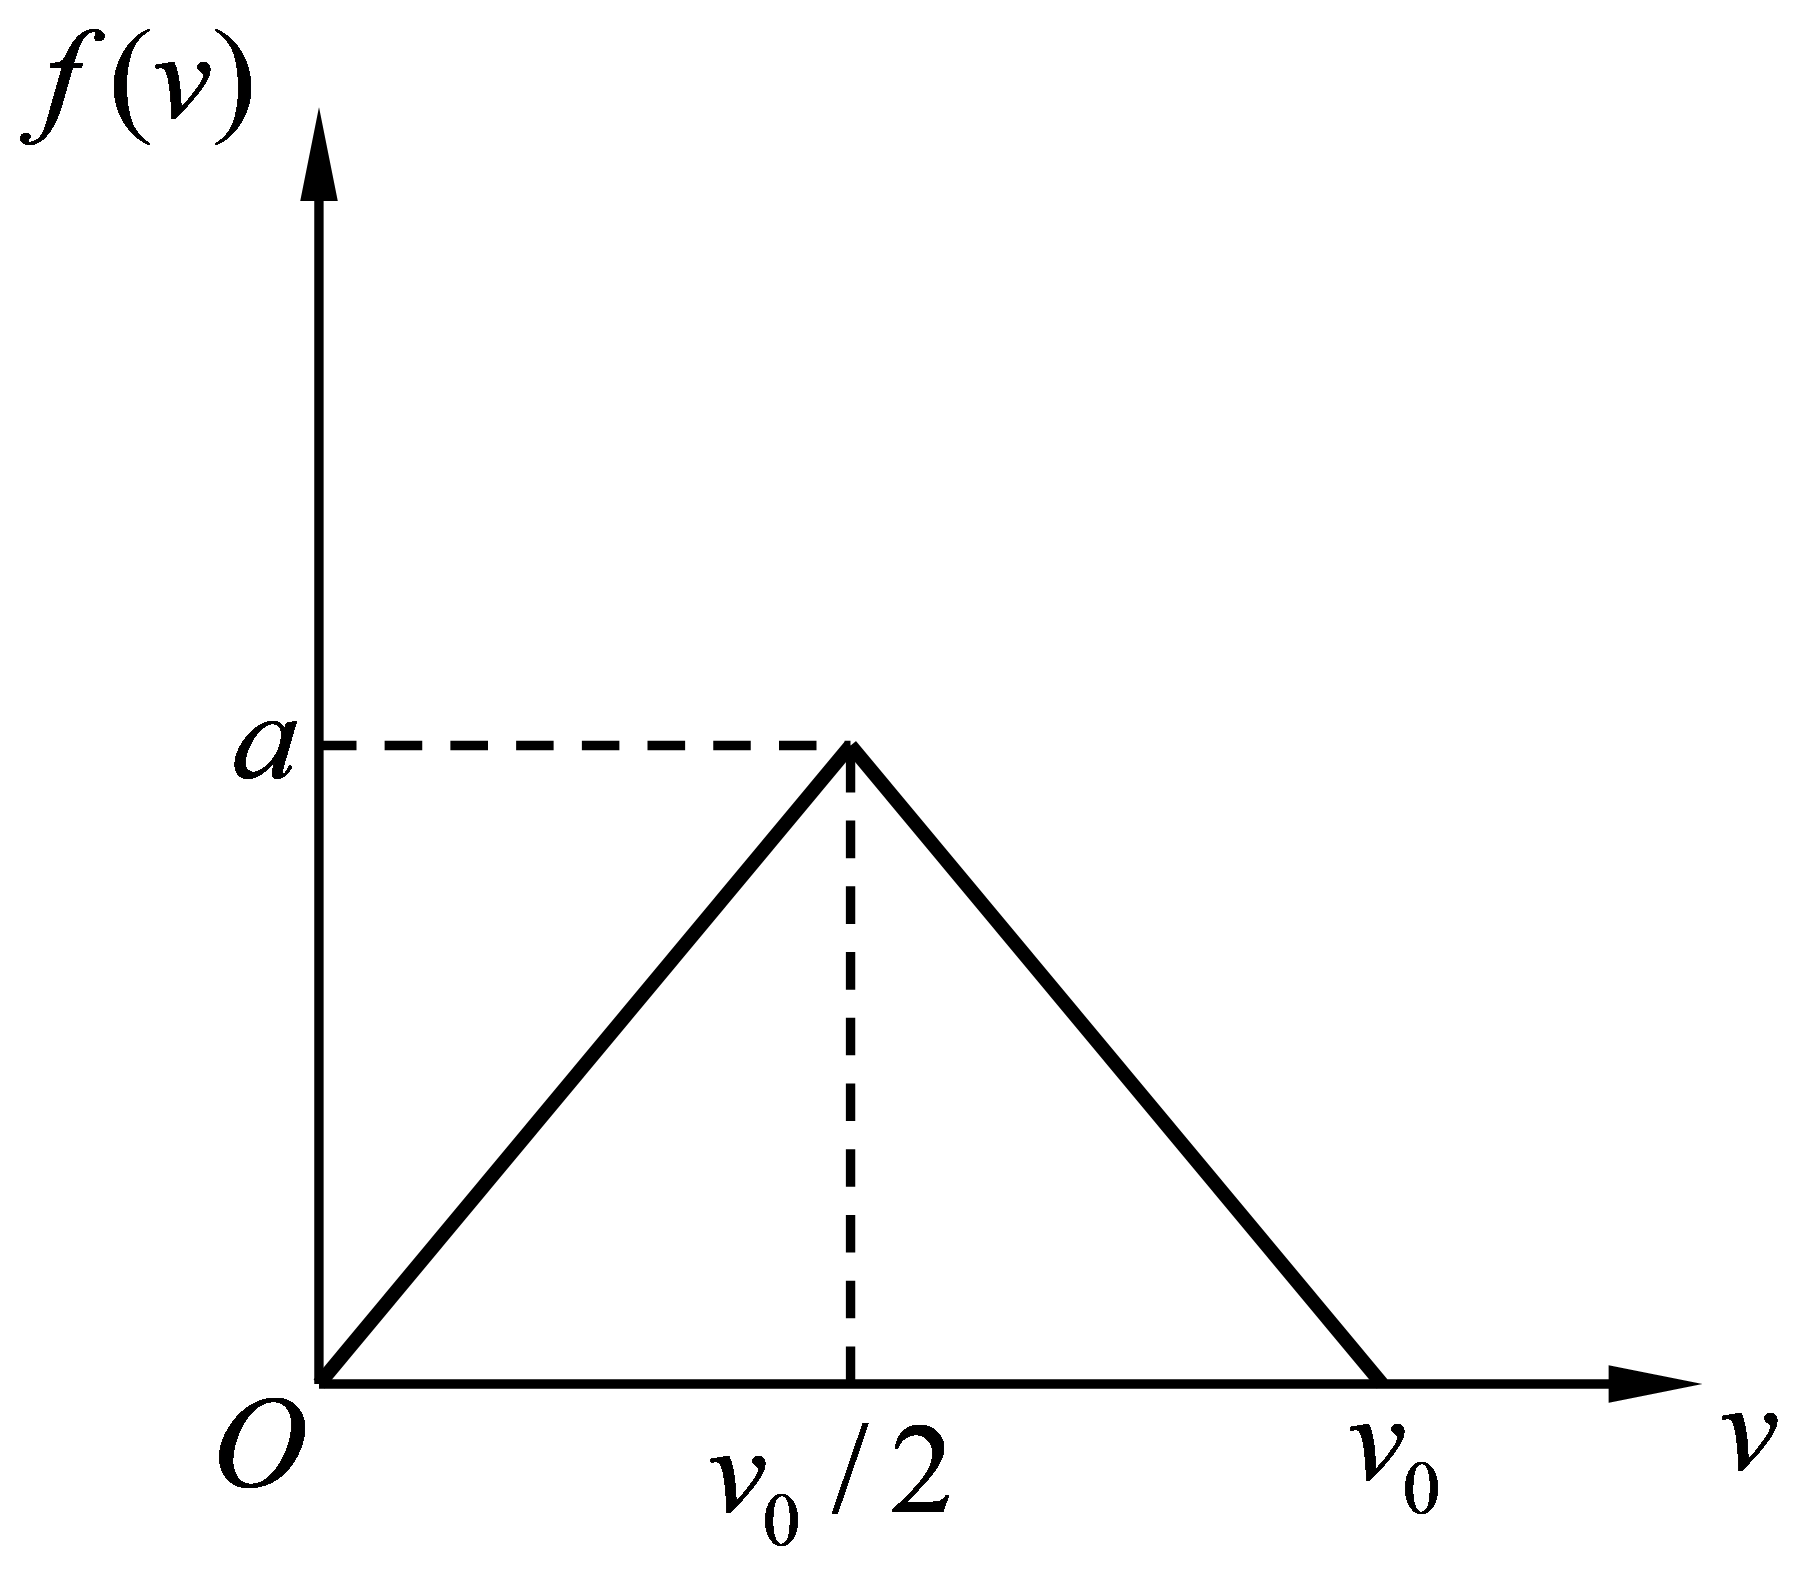
\includegraphics[width=5cm,height=4cm,keepaspectratio]{figures/image22.png}\par}\medskip

\begin{enumerate}
\def\labelenumi{\arabic{enumi}.}
\item
  \[a = ?\]
\item
  分子的最概然速率\(v_{p} = ?\)
\item
  速率在\(\left. 0 \right.\sim\frac{v_{0}}{4}\)之间的分子数；
\item
  分子的平均平动动能。
\end{enumerate}

5．（20 分）

分子被约束在 xy 平面内运动，已知分子速度在\(\left. v_{x} \right.\sim v_{x} + \text{d}v_{x}\)、\(\left. v_{y} \right.\sim v_{y} + \text{d}v_{y}\)内的分子数占总分子数的百分比为

\[\frac{dN_{\overset{\rightarrow}{v}}}{N} = \frac{m}{2\pi kT}e^{- \frac{m(v_{x}^{2} + v_{y}^{2})}{2kT}}dv_{x}dv_{y}\]

式中\(m\)为分子质量，\(T\)为系统温度，\(k\)为玻尔兹曼常数。试求：

\begin{enumerate}
\def\labelenumi{\arabic{enumi}.}
\item
  分子速率在\(\left. v \right.\sim v + \text{d}v\)内的分子数占总分子数的百分比；
\item
  分子平均平动动能（\(\varepsilon = \frac{1}{2}mv^{2}\)）在\(\left. \varepsilon \right.\sim\varepsilon + \text{d}\varepsilon\)内的分子数占总分子数的百分比；
\item
  分子的平均平动动能。
\end{enumerate}

6.（14 分）

设地球大气可近似看成是等温的，温度为 20\textsuperscript{0}C，海平面上的气压\emph{p}\textsubscript{0}=1.0atm，今测得某山顶上的大气压\emph{p}=0.9atm。

（1）分别求出海平面和山顶上的空气密度（单位体积的空气质量）；

（2）山的高度约为多少？

（设空气的平均分子量为 29）

\end{document}
